\section{Data Acquisition and Manipulation}


\subsection{The Human Connectome Project (\textit{HCP})}

\begin{frame}
\frametitle{The Human Connectome Project (\textit{HCP})}
	\begin{itemize}
		\uncover<1->{\item Five-year effort to characterize brain connectivity, function\\and their variability in healthy adults}
		\uncover<2->{\item Multiple imaging modalities: dMRI, r-fMRI,\\t-fMRI, T1w and T2w MRI, MEG, and EEG}
		\uncover<3->{\item 1200 subjects, 300 sibships mostly including\\a mono- or di-zygotic twin pair}
	\end{itemize}
\end{frame}

%\begin{frame}
%\frametitle{HCP Image Acquisition Schematic Summary}
	%\begin{figure}
	%	\centering
	%	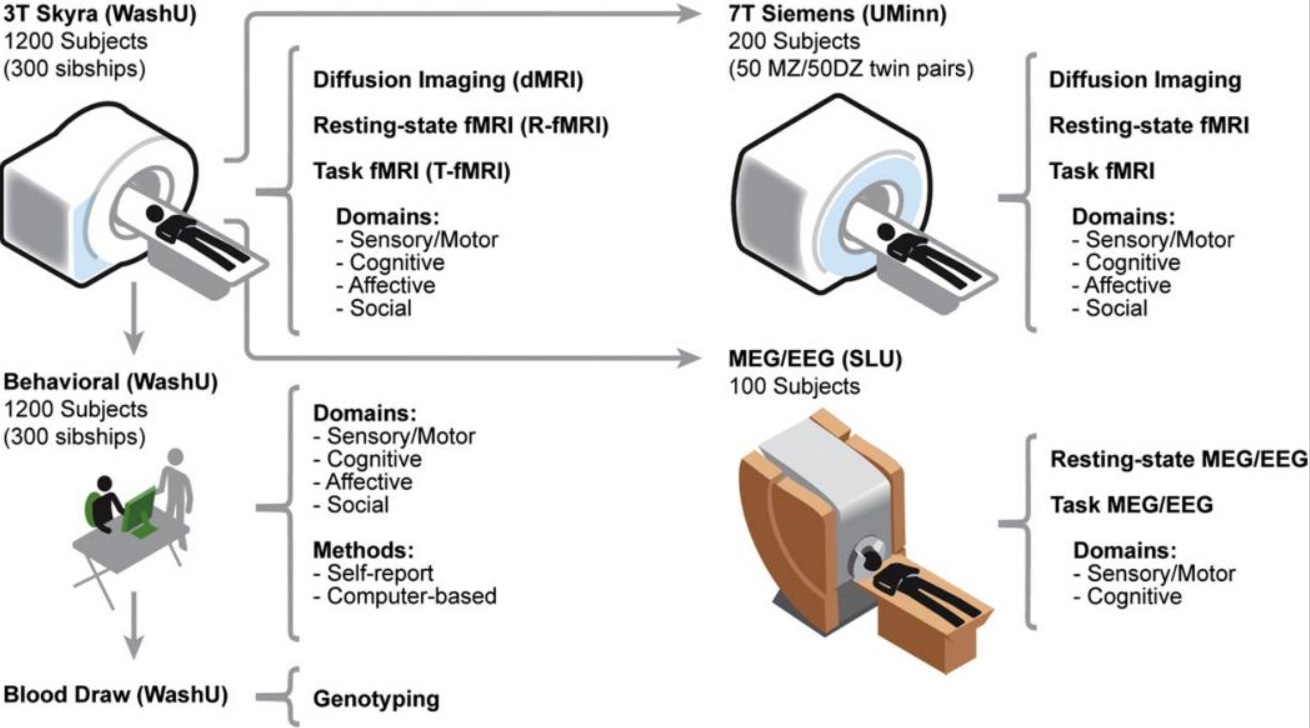
\includegraphics[width=0.98\textwidth]{assets/HCP_plan.png}
	%	\caption*{HCP Image Acquisition Schematic Summary}
	%\end{figure}
%\end{frame}


\subsection{Task-fMRI Battery of the HCP}

\begin{frame}
\frametitle{Task-fMRI Battery of the HCP}
	\text{Neural systems targeted by the tests:}
	\vspace{0.8cm}
	\begin{itemize}
		\item Visual and Somatosensory-Motor Systems
		\item \textbf{Category-Specific Representation}
		\item Language Function (semantic and phonological processing)
		\item Attention Systems
		\item \textbf{Working Memory/Cognitive Control System}
		\item Emotion Processing
		\item Decision-Making/Reward Processing
		\item Episodic Memory Systems
	\end{itemize}
\end{frame}

\begin{frame}
\frametitle{Working Memory Task}
	\begin{columns}
		\begin{column}{0.5\textwidth}
			\begin{itemize}
				\uncover<1->{\item Subjects presented with blocks of trials that consisted of pictures of places, tools, faces, and body parts}
				\uncover<2->{\item N-Back paradigm was utilized}
				\uncover<3->{\item Every 2 blocks separated\\by a fixation period}
				\uncover<4->{\item 8 blocks per run,\\2 runs per subject}
			\end{itemize}
		\end{column}

		\begin{column}{0.49\textwidth}
				\begin{figure}
					\centering
					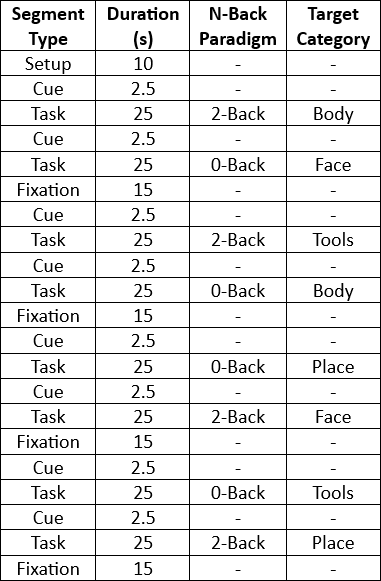
\includegraphics[width=\textwidth, height=6cm]{assets/WM_mat.png}
					\caption*{Sequence of WM Events}
				\end{figure}
		\end{column}
	\end{columns}	
\end{frame}


\subsection{Analysis of fMRI Signal}


\begin{frame}
\frametitle{The Hemodynamic Response Function}
	\begin{columns}
		\begin{column}{0.5\textwidth}
			\begin{itemize}
				\uncover<1->{\item Impulse stimulus produces\\acute hemodynamic response function (\textit{HRF})}
				\uncover<2->{\item Lasting stimulus produces boxcar HRF}
				\uncover<3->{\item HRF shape can be modelled with a Gamma Distribution}
			\end{itemize}
		\end{column}

		\begin{column}{0.49\textwidth}
			\only<1>{	
				\begin{figure}
					\centering
					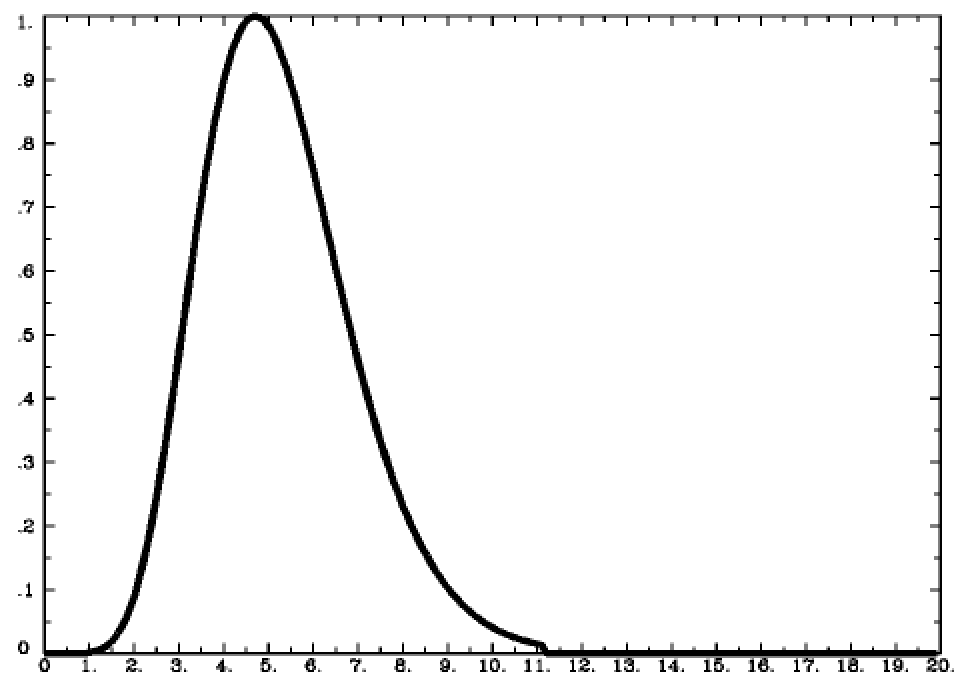
\includegraphics[width=\textwidth, height=6cm]{assets/single_HRF.jpg}
					\caption*{Illustration of Acute HRF.}
				\end{figure}
				}
			\only<2>{	
				\begin{figure}
					\centering
					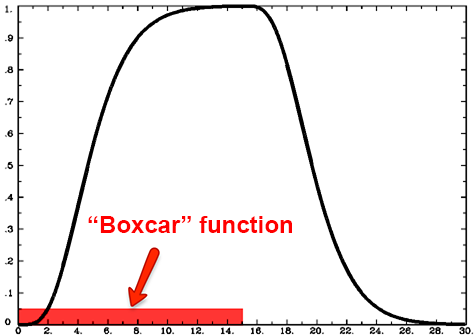
\includegraphics[width=\textwidth, height=6cm]{assets/box_HRF.jpg}
					\caption*{Illustration of Boxcar HRF.}
				\end{figure}
				}
			\only<3>{	
				\begin{figure}
					\centering
					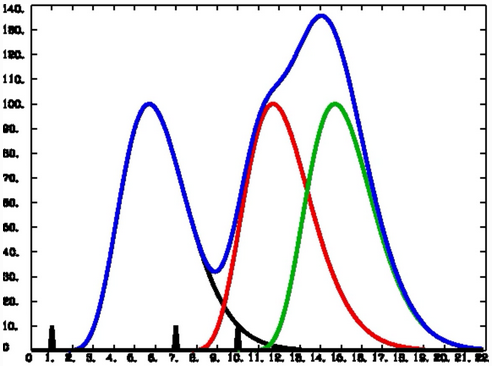
\includegraphics[width=\textwidth, height=6cm]{assets/overlap_HRF.png}
					\caption*{HRF Overlap and Fitting.}
				\end{figure}
				}
		\end{column}
	\end{columns}	
\end{frame}

% potential gif of hrf scaling

\begin{frame}
\frametitle{Analysis Process Overview}
	\begin{itemize}
		\uncover<1->{\item General Linear Model fitting to the BOLD signal time-series}
		\uncover<2->{\item Original explanatory variables (\textit{EV}) defined by the experiment}
		\uncover<3->{\item Beta-weights corresponding to each EV}
		\uncover<4->{\item Contrast of parameter estimates (\textit{COPE}) selected by researcher}
	\end{itemize}
	\begin{figure}
		\centering
		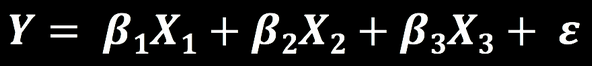
\includegraphics[width=\textwidth]{assets/glm.png}
	\end{figure}
\end{frame}

\begin{frame}
\frametitle{Unprocessed BOLD Time-Series.}
	\begin{itemize}
		\item Unprocessed BOLD Time-Series
	\end{itemize}
	\begin{figure}
		\centering
		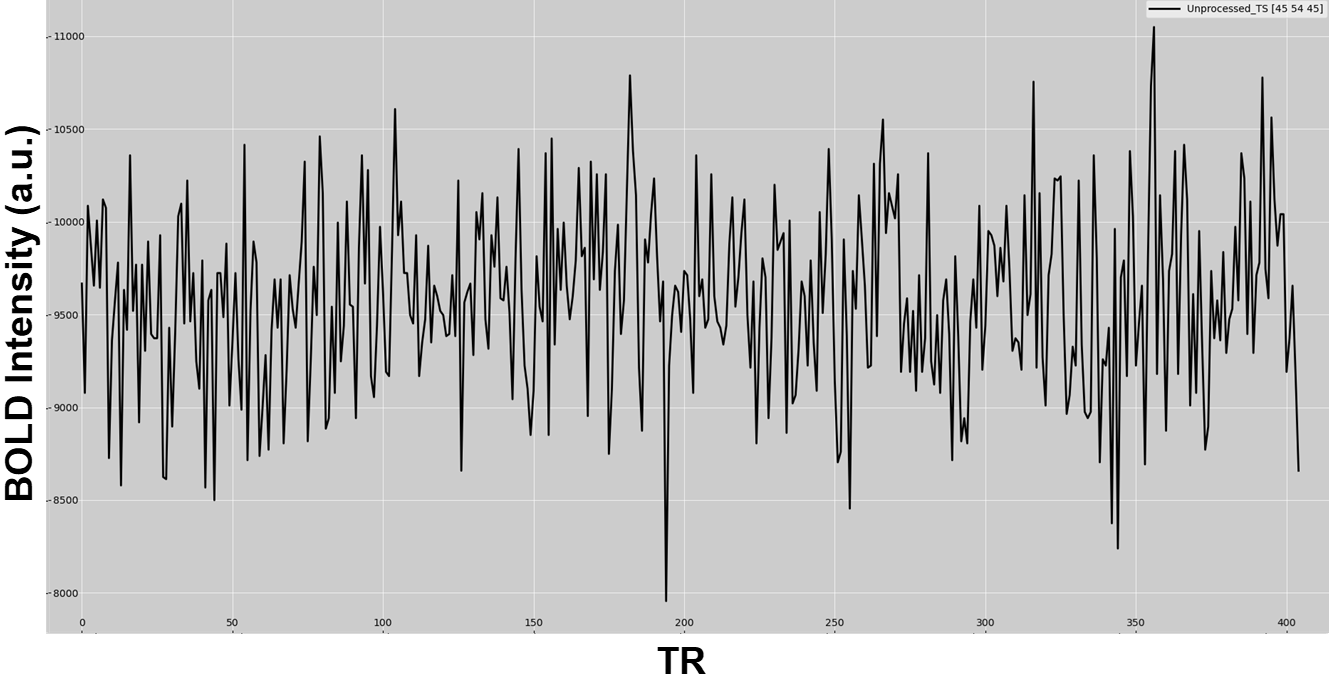
\includegraphics[width=\textwidth]{assets/unproc.png}
	\end{figure}
\end{frame}

\begin{frame}
\frametitle{Preprocessed BOLD Time-Series.}
	\begin{itemize}
		\item Unprocessed Versus Preprocessed BOLD Time-Series
	\end{itemize}
		\begin{figure}
			\centering
			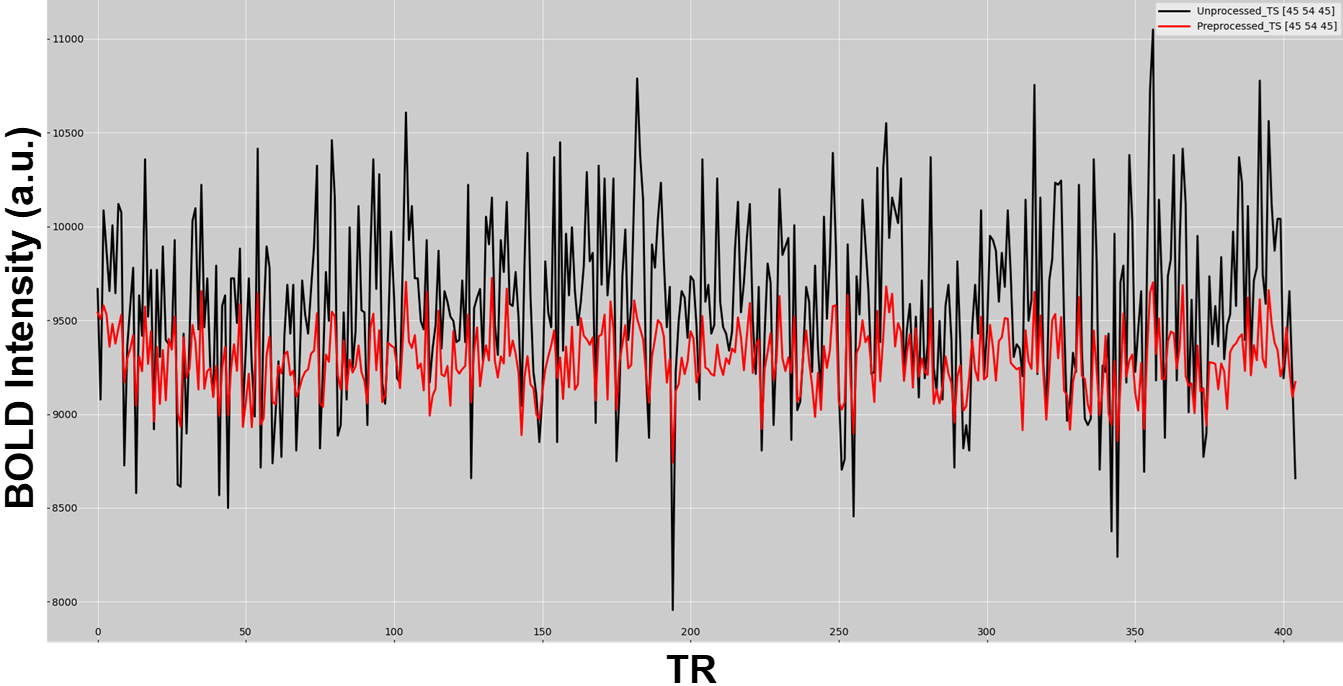
\includegraphics[width=\textwidth]{assets/preproc_and_unproc.png}
		\end{figure}
\end{frame}

\begin{frame}
\frametitle{Fitted BOLD Time-Series.}
	\begin{itemize}
		\item Preprocessed Versus Fitted BOLD Time-Series
	\end{itemize}
	\begin{figure}
		\centering
		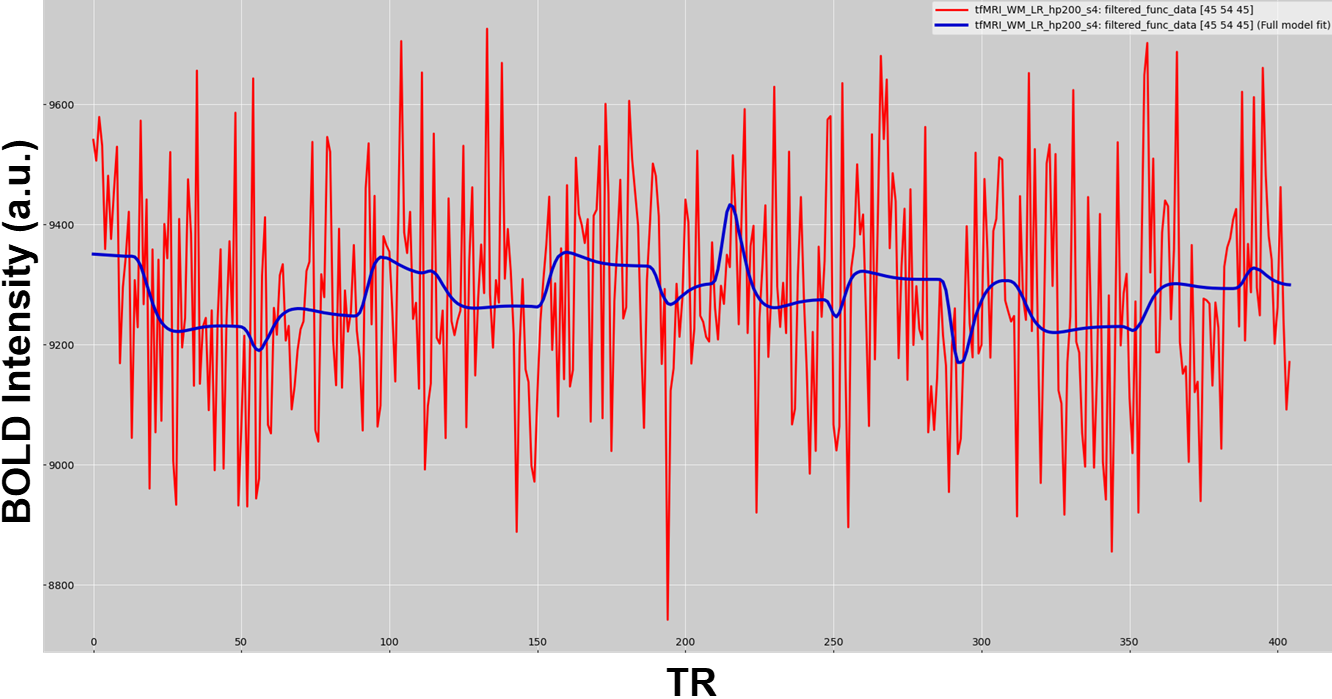
\includegraphics[width=\textwidth]{assets/fitted_and_preproc.png}
	\end{figure}
\end{frame}

%\begin{frame}
%\frametitle{Fitted BOLD Time-Series.}
%	\begin{itemize}
%		\item COPE configuration for estimating HRF beta weights for stimuli\\belonging to specific category and N-Back paradigm
%	\end{itemize}
%	\begin{figure}
%		\centering
%		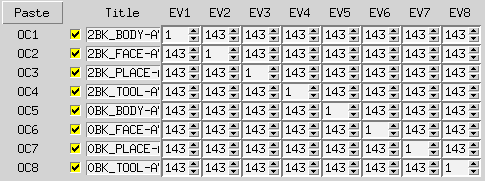
\includegraphics[width=\textwidth]{assets/COPEs_4C.png}
%	\end{figure}
%\end{frame}